%% Method/measurement-pipeline overview for "Two Ways a Design Fails".
%% Standalone flat-vector; build: pdflatex fig_pipeline_concept.tex
\documentclass[border=6pt]{standalone}
\usepackage{times}
\usepackage{tikz}
\usetikzlibrary{arrows.meta,positioning,fit,backgrounds,calc,shapes.geometric}
\definecolor{okgreen}{HTML}{009E73}
\definecolor{okred}{HTML}{D55E00}
\definecolor{okblue}{HTML}{0072B2}
\definecolor{okgray}{HTML}{6E6E6E}
\definecolor{panelbg}{HTML}{EFF4FA}
\definecolor{outbg}{HTML}{FBF0E8}
\begin{document}
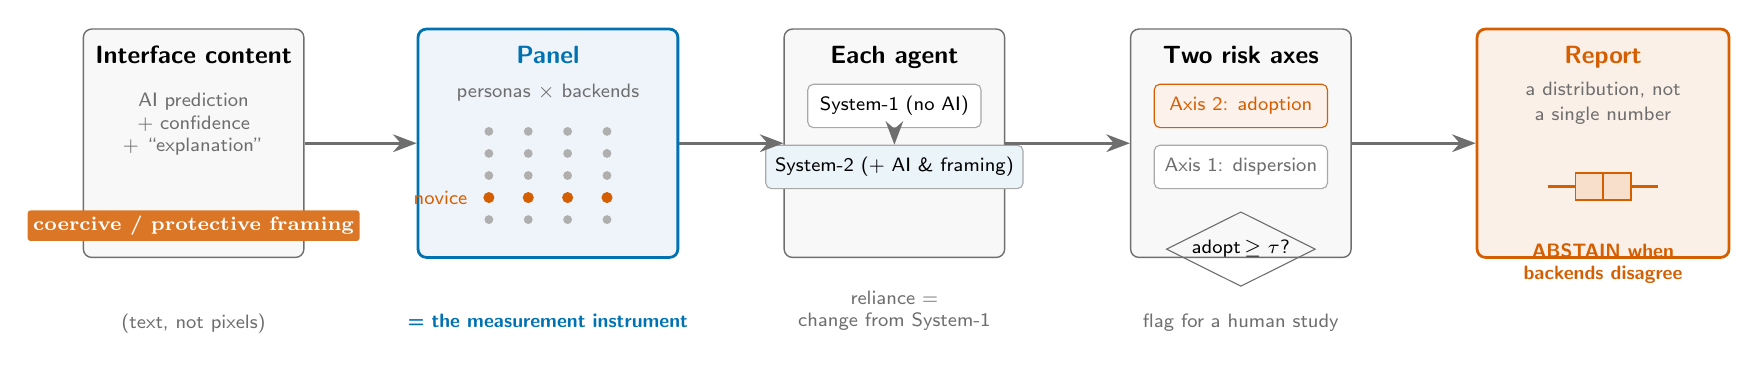
\begin{tikzpicture}[font=\sffamily,>={Stealth[length=3mm]},
  stage/.style={draw=okgray,rounded corners=3pt,fill=okgray!5,line width=0.5pt,
                minimum width=2.8cm,minimum height=2.9cm,align=center,inner sep=3pt},
  head/.style={font=\sffamily\bfseries\small},
  lab/.style={font=\sffamily\small},
  tiny/.style={font=\sffamily\scriptsize,text=okgray},
  chip/.style={draw=okgray!60,rounded corners=2pt,fill=white,line width=0.4pt,
               minimum width=2.2cm,minimum height=0.55cm,font=\sffamily\scriptsize}]

% ===== Stage 1: interface content =====
\node[stage] (s1) at (0,0) {};
\node[head,anchor=north] at ([yshift=-3pt]s1.north) {Interface content};
\node[tiny,anchor=north,align=center] at ([yshift=-20pt]s1.north) {AI prediction\\+ confidence\\+ ``explanation''};
\node[anchor=south,fill=okred!85,text=white,font=\scriptsize\bfseries,rounded corners=1pt,
      inner sep=2pt,minimum width=2.3cm] at ([yshift=6pt]s1.south) {coercive / protective framing};
\node[tiny,anchor=north] at (0,-2.05) {(text, not pixels)};

% ===== Stage 2: panel = personas x backends (the instrument) =====
\node[stage,draw=okblue,line width=1pt,fill=panelbg,minimum width=3.3cm] (s2) at (4.5,0) {};
\node[head,anchor=north,text=okblue] at ([yshift=-3pt]s2.north) {Panel};
\node[tiny,anchor=north] at ([yshift=-17pt]s2.north) {personas $\times$ backends};
\foreach \r in {0,...,4}{\foreach \c in {0,...,3}{
  \pgfmathsetmacro{\xx}{3.75+\c*0.5}\pgfmathsetmacro{\yy}{0.15-\r*0.28}
  \ifnum\r=3 \fill[okred](\xx,\yy)circle(2pt);\else\fill[okgray!55](\xx,\yy)circle(1.6pt);\fi}}
\node[tiny,anchor=east,text=okred] at (3.6,0.15-3*0.28) {novice};
\node[font=\sffamily\bfseries\scriptsize,text=okblue,anchor=north] at (4.5,-2.05) {= the measurement instrument};

% ===== Stage 3: two-stage decision =====
\node[stage] (s3) at (8.9,0) {};
\node[head,anchor=north] at ([yshift=-3pt]s3.north) {Each agent};
\node[chip,anchor=north] (sysa) at ([yshift=-20pt]s3.north) {System-1 (no AI)};
\node[chip,anchor=north,fill=okblue!8] (sysb) at ([yshift=-6pt]sysa.south) {System-2 (+ AI \& framing)};
\draw[->,okgray,line width=0.6pt] (sysa.south) -- (sysb.north);
\node[tiny,anchor=north,align=center] at (8.9,-1.75) {reliance =\\change from System-1};

% ===== Stage 4: two axes + decision =====
\node[stage] (s4) at (13.3,0) {};
\node[head,anchor=north] at ([yshift=-3pt]s4.north) {Two risk axes};
\node[chip,anchor=north,draw=okred,fill=okred!8,text=okred] (ax2) at ([yshift=-20pt]s4.north) {Axis 2: adoption};
\node[chip,anchor=north,text=okgray] (ax1) at ([yshift=-6pt]ax2.south) {Axis 1: dispersion};
\node[diamond,draw=okgray,aspect=2,inner sep=1pt,font=\sffamily\scriptsize,anchor=north,align=center]
      at ([yshift=-8pt]ax1.south) {adopt\,$\ge\tau$?};
\node[tiny,anchor=north] at (13.3,-2.05) {flag for a human study};

% ===== Stage 5: output = distribution + abstain =====
\node[stage,draw=okred,line width=1pt,fill=outbg,minimum width=3.2cm] (s5) at (17.9,0) {};
\node[head,anchor=north,text=okred] at ([yshift=-3pt]s5.north) {Report};
\node[tiny,anchor=north] at ([yshift=-16pt]s5.north) {a distribution, not};
\node[tiny,anchor=north] at ([yshift=-25pt]s5.north) {a single number};
% mini box-plot glyph
\draw[okred,line width=0.8pt] (17.2,-0.55)--(18.6,-0.55);
\filldraw[fill=okred!20,draw=okred,line width=0.7pt] (17.55,-0.72) rectangle (18.25,-0.38);
\draw[okred,line width=0.9pt] (17.9,-0.72)--(17.9,-0.38);
\node[font=\sffamily\bfseries\scriptsize,text=okred,anchor=north,align=center] at (17.9,-1.15)
      {ABSTAIN when\\backends disagree};

% ===== arrows =====
\draw[->,okgray,line width=1pt] (s1.east)--(s2.west);
\draw[->,okgray,line width=1pt] (s2.east)--(s3.west);
\draw[->,okgray,line width=1pt] (s3.east)--(s4.west);
\draw[->,okgray,line width=1pt] (s4.east)--(s5.west);

\end{tikzpicture}
\end{document}
